\section{Background and Motivation \label{background}}
\subsection{Motivation}
As we mentioned in the section \ref{intro}, a key goal of our efforts  is to develop methods to use DL to help predict properties of molecules from first principles. That is, rather than trying to engage in complex and often {\em intuition-based} feature engineering effort, we want to use basic and readily available chemical and physical information as input to the models. The rationale behind this is that deep neural networks have been shown to excel at using early layer in the network as {\em feature generators} that are then used by mid and late layers in the network. Publicly available database, such as PubChem (REF) and OQMD (REF) provide the foundational information from which to draw the set of basic features to serve as input  to the model. These databases provide a) chemical properties, b) physical properties, c) spatial structures of molecules, 2D imaging on 
\subsection{ML Methods Used}
\subsection{SMILES}
    \begin{itemize}
        \item Simplified Molecular Input Line Entry System (SMILES) is a line notation for describing chemical structures in a way that is easier for computers to interpret. 
        \item It consists of a series of characters containing no spaces that uses a simple vocabulary and a few grammar rules.
        \item In this notation atoms are represented by their atomic symbol while bonds and branches are represented by special characters.
        \item Unfortunately based exclusively on the basic rules for generating a SMILES string there can exist more than one way to represent a single compound.
        \item To help assign just one representation per structure and permit consistency a canonicalization algorithm is typically used by databases. This algorithm's job is to generate and assign one specific SMILES string for each structure.
        \item In our dataset these are called canonical SMILES.
        \item Another type of SMILES string that are often used and are also available in our dataset are isometric SMILES. These include isotopic specifications of a chemical structure.
    \end{itemize}
    \subsubsection{SMILES Rules}
        \begin{enumerate}
            \item Atoms are represented by their atomic symbol and are enclosed in brackets []. The organic subset can be written without brackets, these include: B, C, N, O, S, F, Cl, Br, and I. Brackets can also be used to remove ambiguities about the charge of the atom. 
            \item Bonds are represented as follows:
            \begin{itemize}
                \item[$-$] single bond
                \item[$=$] double bond
                \item[$\#$] triple bond
                \item[$.$] disconnected structure
            \end{itemize}
            \textbf{Note:} Single bonds can be omitted as shown in Figures \ref{fig:smile-examples} and \ref{fig:smile-examples2}.
            \item Branches are represented with parenthesis, ().
            \item Cyclic structures or carbon rings are represented with digits. The first digit is the beginning of the rings and the matching digit that follows is when the ring closes. This can also be observed in Figures \ref{fig:smile-examples} and \ref{fig:smile-examples2}.
        \end{enumerate}
    \subsubsection{Correspondence between the 2D structure and a SMILES}
        \begin{itemize}
            \item In Figure \ref{fig:smile-examples} we can see two chemical models each with a cyclic cycle.
            \item Each edge and end of the 2D model represent a carbon and in both the model and SMILES the hydrogen is omitted as it is assumed that they fill any missing bonds.
            \item Notice in Figure \ref{fig:smile-examples} the leftmost figure its SMILES has a double bond which is illustrated in the 2D model. It is then followed by a digit indicating that the next sequence is for a cyclic structure. 
            \item So in this first figure we have that it starts at a carbon which is the starting point for a cyclic cycle and the cycle starts with a double bond. 
            \item In the rightmost image we see similarly that it starts with a carbon, in this case it is the one located at the leftmost edge of the triangle. This carbon starts the cycle that includes an oxygen atom and note that when the cycle closes the next part of the SMILES continues from the initial carbon.
            \item In Figure \ref{fig:smile-examples2} we can observe a more detailed example that better illustrates how the various rules come together to represent what we see in the 2D model.
            \item The initial red 'C' in the SMILES is shown in the 2D structure with the red circle. That is our starting position. 
            \item This is followed by a '1' implying that the red 'C' belongs in a carbon ring and will be treated as the starting point of it. And the carbon ring closes at the orange 'C' since this is followed by the second '1'.
            \item We can notice as well that the orange 'C' also forms part of a branch as it is enclosed in a parenthesis. The entire branch can be observed in the 2D model inside the purple circle.
            \item Finally the green text of the SMILES can be seen inside the green circle. Notice that it is attached to the first carbon of the SMILES (red 'C'). 
        \end{itemize}
    
    \begin{figure}[h]
        \centering
        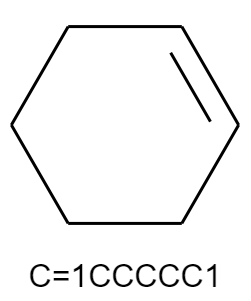
\includegraphics[width=0.25\textwidth]{figures/Smiles-Smile1.png}
        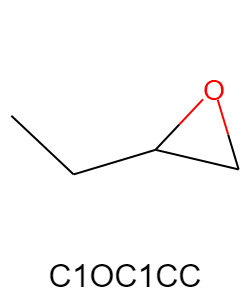
\includegraphics[width=0.25\textwidth]{figures/Smiles-Smile2.png}
        \caption{Example of 2 chemical structures and their respective SMILES}
        \label{fig:smile-examples}
    \end{figure}
    \begin{figure}[h]
        \centering
        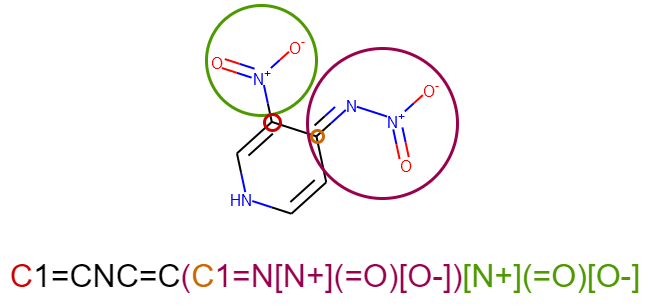
\includegraphics[width=0.5\textwidth]{figures/Smiles-Smile3.png}
        \caption{Example of how each part of the SMILES string corresponds to the 2D model of the chemical structure.}
        \label{fig:smile-examples2}
    \end{figure}
\subsection{Applying NLP Ideas}
